\begin{figure}[htbp]
    \begin{subfigure}{\textwidth}
    \centering
    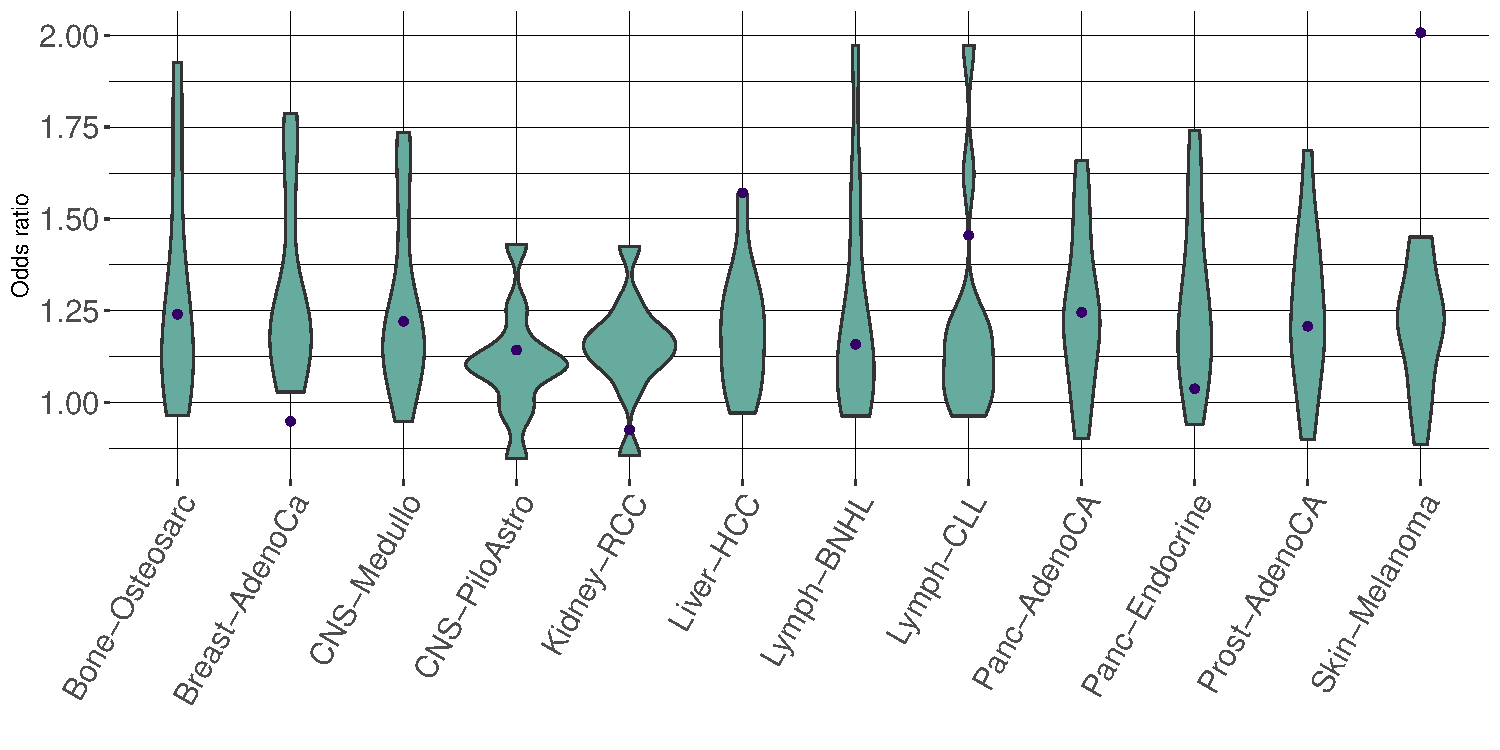
\includegraphics[scale=0.6]{graphics/mixed_or_violin.pdf}
    \caption{}
    \label{fig:mixed_or_violin}
    \end{subfigure}
    ~
    \begin{subfigure}{\textwidth}
    \centering
    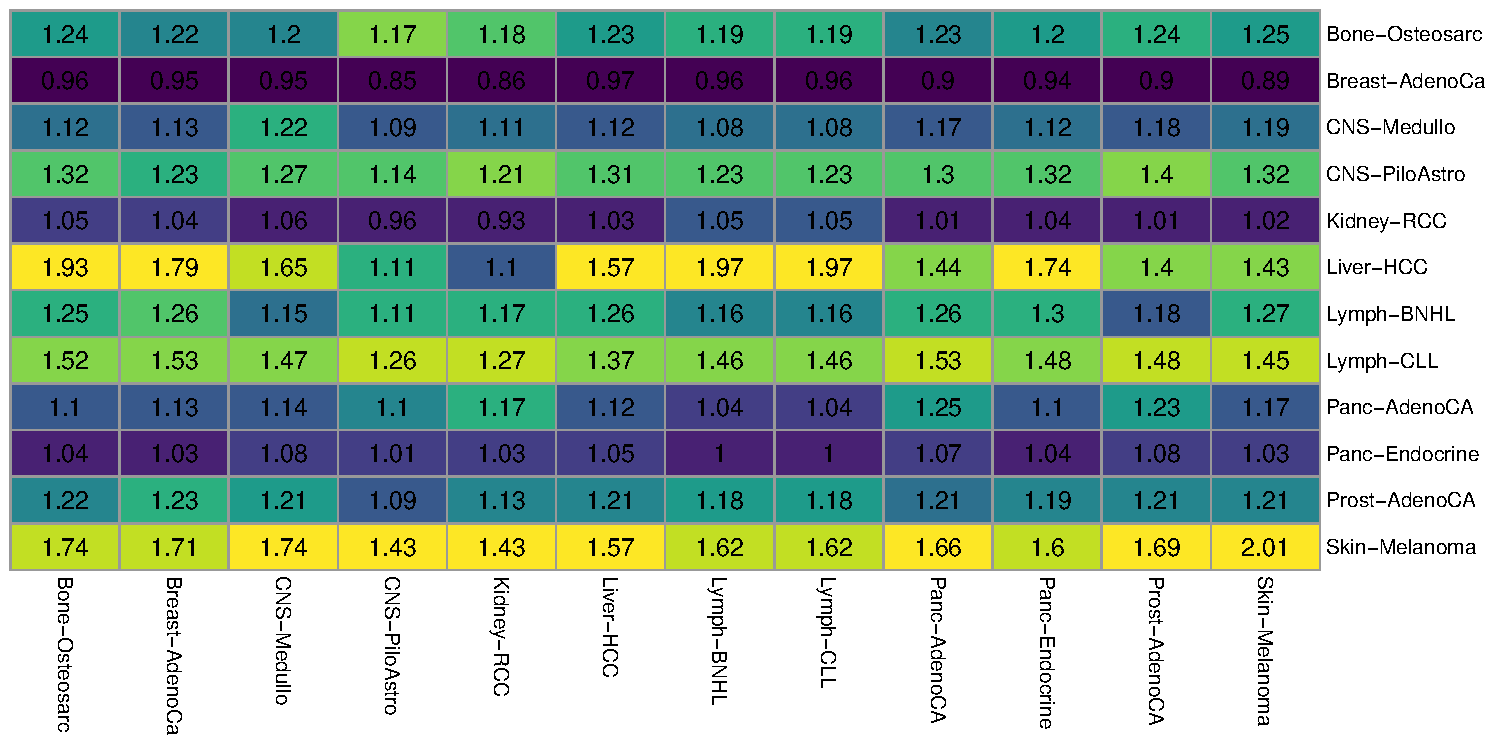
\includegraphics[scale=0.6]{graphics/mixed_or_heatmap.pdf}
    \caption{}
    \label{fig:mixed_or_heatmap}
    \end{subfigure} \\
    \vspace{0.5cm}

    \caption{\textbf{Mutations tend to be found in closed chromatin regions.} Different cancers differ in the distribution of mutations across the genome. Here chromosome 12 is shown. (a) Skin-Melanoma (b) Kidney-RCC (c) Liver-HCC (d) Panc-AdenoCA. The green bar below the x-axis indicates hypersensitivity regions, the gap indicates closed chromatin regions of the original cell types. The vertical dotted line indicates the position of the centromere.}
    \label{fig:mixed_or}
\end{figure}